\section{Композиция}

\label{sec:composition}

Ядро строится вокруг трёх компонент: \textit{Distributions}, \textit{Families} и \textit{Transformations}. 
Они объединены общей идеей: все вычисления характеристик случайных величин происходят по единым контрактам, а сами компоненты остаются слабо связаны и расширяемы.

\subsection{Роли компонент}

\paragraph{Families.}
Families отвечает за параметризацию и рождение конкретных распределений. 
Под параметризацией понимается множество имён параметров, а под параметрами --- отображение этих имён в значения. 
Поддерживается несколько параметризаций для одной и той же семьи, однако все вычисления выполняются через базовую параметризацию. 
Перед любыми вычислениями параметры приводятся к базовой форме, чтобы остальные компоненты работали с единым представлением. 
Families сохраняет смысловую целостность параметров, их допустимость и область определения будущего распределения.

\paragraph{Distributions.}
Distributions --- единая поверхность доступа к характеристикам распределений и точка их композиции. 
Компонента материализует распределение, зная его семью и параметры, и предоставляет согласованный интерфейс к характеристикам: функциям распределения, плотности, квантилям, моментам и т.\,д. 
Distributions не решает, \emph{как} именно получена та или иная характеристика; она лишь координирует вычисление по зависимостям и контрактам, в том числе для составных объектов, которые появились в результате преобразований.

\paragraph{Transformations.}
Transformations фиксирует операции над распределениями и правила пересчёта характеристик после этих операций. 
Сюда попадают преобразования вида «аффинное», «сдвиг и масштаб», «сумма/микс», «свёртка», «обрезка (truncation)», «монотонные отображения» и другие композиции. 
Компонента описывает, \emph{какие} характеристики нового распределения можно выразить через характеристики исходных и в каком порядке они должны вычисляться.
На момент написания модуль проектно важен, но ещё не реализован; он задаёт общий язык описания преобразований и обеспечивает единообразную логику пересчёта поддержек, моментов, квантилей и прочих характеристик при переходе к результату преобразования.

\subsection{Поток данных и точки соприкосновения}

Рабочий цикл выглядит просто. Пользователь выбирает семью и задаёт параметры в удобной для него параметризации. 
Families приводит параметры к базовой форме и передаёт контекст в Distributions. 
Когда требуется характеристика, Distributions строит локальный граф зависимостей для этого запроса. 
Если характеристика получена применением преобразования, узлы этого графа добавляются модулем Transformations, а рёбра указывают, какие характеристики исходных распределений нужны для пересчёта. 
Таким образом, вычисления идут от стандартизованных параметров через согласованные правила преобразований к запрошенной характеристике результата.

\subsection{Границы и контракты}

Межкомпонентное взаимодействие опирается на несколько устойчивых сущностей: 
базовая параметризация, область значения случайной величины (support), именованный реестр характеристик и спецификация преобразований. 
Компоненты не разделяют внутреннее состояние и обмениваются только тем, что необходимо для вычисления. 
Это позволяет добавлять новые семьи и новые преобразования без изменения существующих модулей, сохраняя обратную совместимость.

\subsection{Композиционные свойства}

Композиция прозрачна: результат преобразования ведёт себя как обычное распределение, подчиняясь тем же контрактам Distributions. 
Порядок вычисления характеристик незначим для внешнего пользователя, так как зависимости и правила вывода зашиты в Transformations. 
Единая базовая параметризация в Families гарантирует сопоставимость результатов при смешении разных источников и представлений параметров.

\begin{figure}[H]
  \centering
  % Замените путь на ваш файл со схемой компонентов.
  % Если у вас PDF/PNG, оставьте только одно расширение
  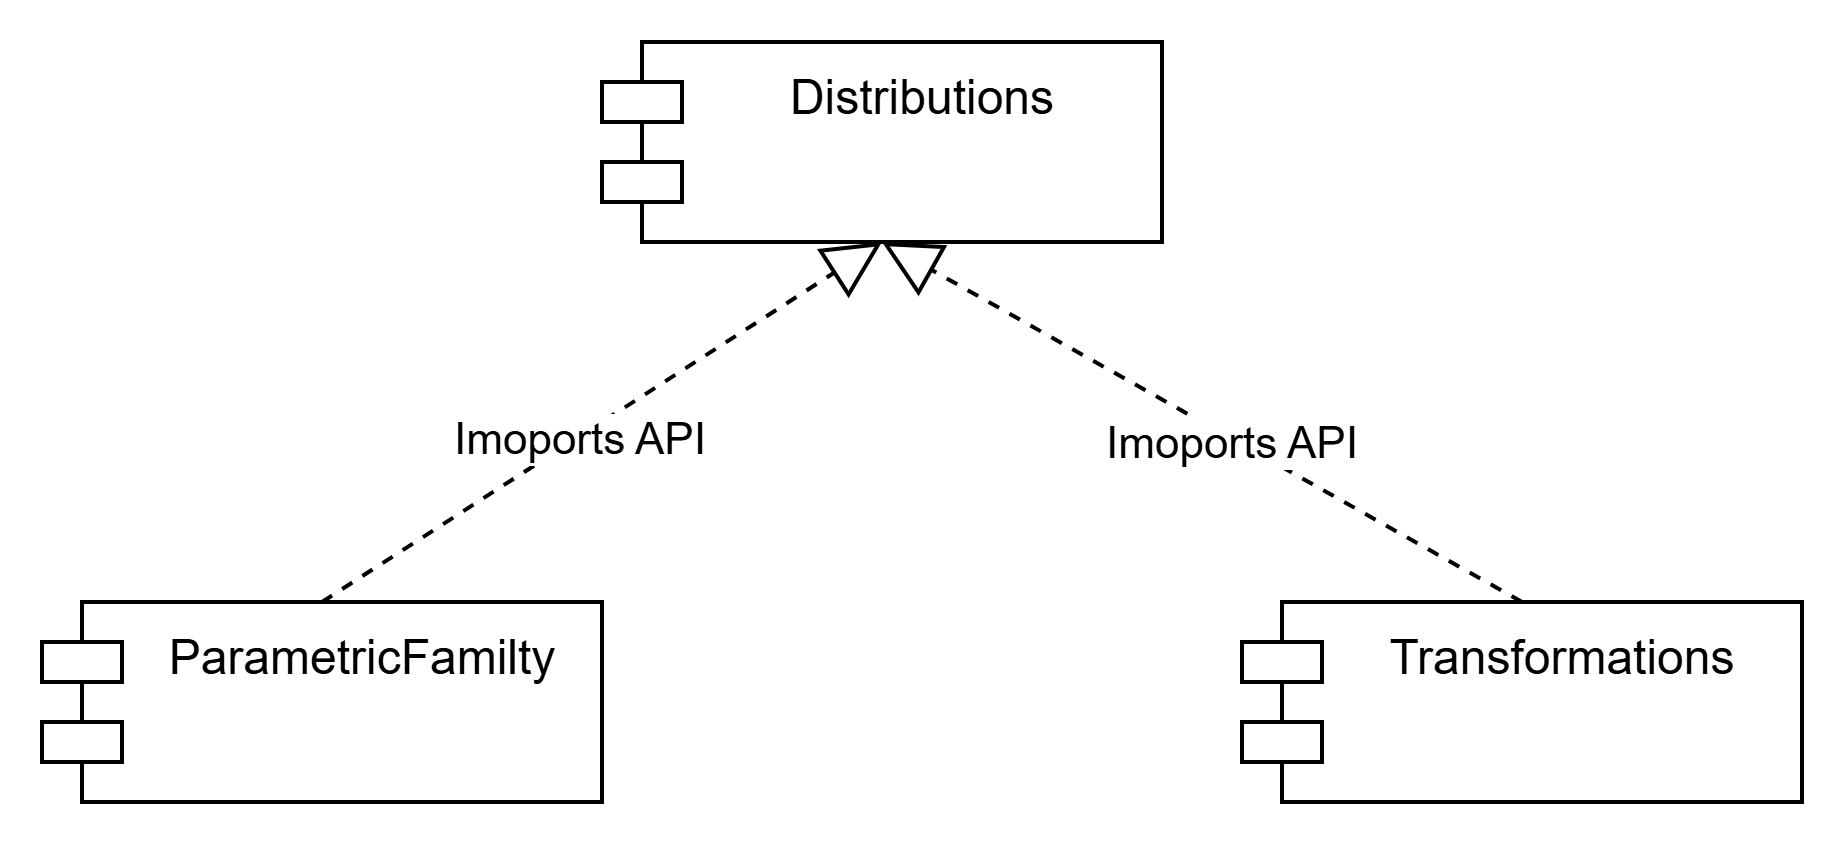
\includegraphics[width=.85\linewidth]{assets/images/Composition.png}
  \caption{Компоненты ядра и их роли в композиции}
  \label{fig:kernel-components}
\end{figure}